% This version of CVPR template is provided by Ming-Ming Cheng.
% Please leave an issue if you found a bug:
% https://github.com/MCG-NKU/CVPR_Template.

%\documentclass[review]{cvpr} 
\documentclass[final]{cvpr}

\usepackage{times}
\usepackage{epsfig}
\usepackage{graphicx}
\usepackage{amsmath}
\usepackage{amssymb}
\usepackage{multirow}


% Include other packages here, before hyperref.

% If you comment hyperref and then uncomment it, you should delete
% egpaper.aux before re-running latex.  (Or just hit 'q' on the first latex
% run, let it finish, and you should be clear). 
\usepackage[pagebackref=true,breaklinks=true,colorlinks,bookmarks=false]{hyperref}


\def\cvprPaperID{2635} % *** Enter the CVPR Paper ID here
\def\confYear{CVPR 2021}
%\setcounter{page}{4321} % For final version only
\pagenumbering{gobble}

\begin{document}
\renewcommand{\arraystretch}{1.1}
%%%%%%%%% TITLE
\title{\Large Title}

\author{Seungmin Lee\\
Seoul National University\\
{\tt\small dltmdals14@snu.ac.kr}
}

\onecolumn
\maketitle

\section{Any Title}

\begin{figure}[t]
	\begin{tabular}{c@{\hskip0.5cm}c}
		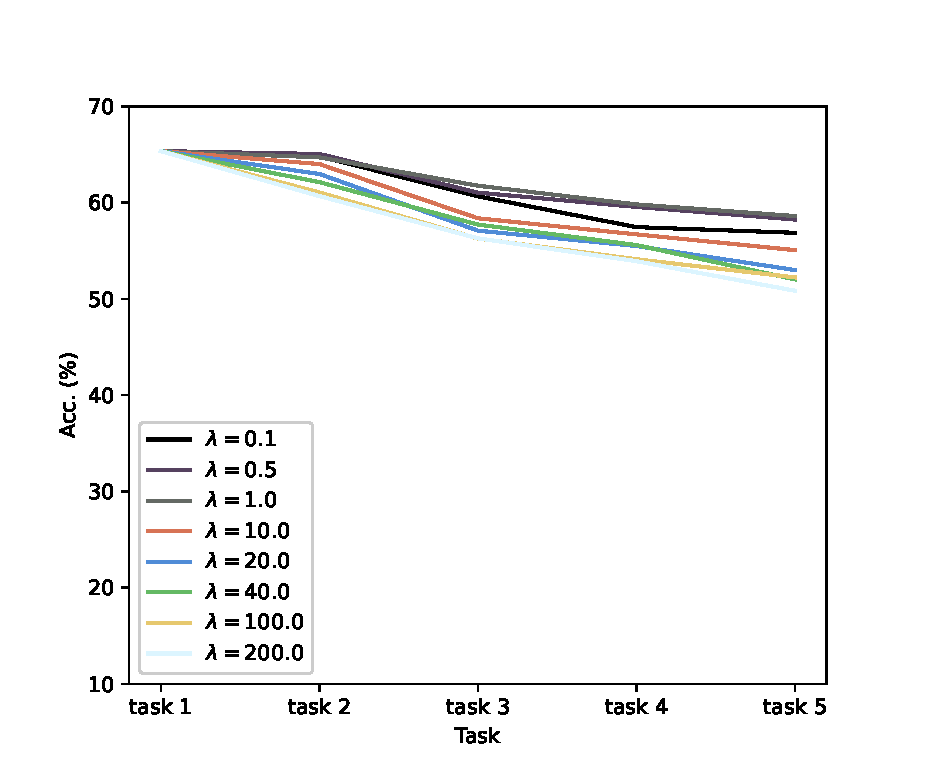
\includegraphics[width=0.5\textwidth]{resources/ewc_CIFAR.eps}&%	
        \includegraphics[width=0.5\textwidth]{resources/l2_CIFAR.eps}\\%
        (a) EWC CIFAR100 & (b) L2 CIFAR100\\
        \includegraphics[width=0.5\textwidth]{resources/ewc_MNIST.eps}&%	
        \includegraphics[width=0.5\textwidth]{resources/l2_MNIST.eps}\\%
		(c) EWC MNIST  & (d) L2 MNIST \\
	\end{tabular}\vspace{0.2cm}
	\caption{some captions}
	\label{fig:tsne}
	% \vspace{-0.4cm}
\end{figure}



{\small
	\bibliographystyle{ieee_fullname}
	\bibliography{egbib}
}

\end{document}
